\chapter{Stage 3a --- Brightness-Constrained Optimum}
\label{ch:stage3a}

\section{Motivation}

Chapter~\ref{ch:r1sweep}'s pure blur-minimization optimum sits well below the range
sunglasses manufacturers and patent filings actually use. Stage 3a asks: does adding a
single, simple brightness (illuminance) floor to the optimization --- \emph{minimize
blur, subject to admitting at least a minimum fraction of full-pupil light} --- close
that gap?

\section{Relative illuminance}

For a single circular pinhole of diameter $a_{hole}$ in front of an eye with natural
(unobstructed) pupil diameter $D_{pupil}$, diffraction redistributes power spatially
but does not destroy it: total transmitted power through the aperture is proportional
to its physical area, not to any diffraction-broadened blur-radius estimate. Once
$a_{hole}$ exceeds $D_{pupil}$, the pupil itself becomes the limiting stop. Relative
illuminance (as a fraction of normal, full-pupil viewing) is therefore the clipped
area ratio
\begin{equation}
E_{rel}(a_{hole}) = \left(\frac{\min(a_{hole}, D_{pupil})}{D_{pupil}}\right)^{2}.
\label{eq:erel}
\end{equation}

\section{The constrained optimization}

For each myopia level $M$, Stage 3a takes the full corrected-optics blur sweep
(Chapter~\ref{ch:r1sweep}), restricts to apertures with $E_{rel}(a_{hole}) \ge T_{min}$,
and reports the aperture within that restricted set that minimizes $r_{EE}(50\%)$ ---
i.e., the smallest-blur aperture that still clears the brightness floor. This report
uses $T_{min}=6.25\%$, the low end of this project's own previously-established
brightness-floor range ($6.25$--$9\%$).

\begin{figure}[htbp]
\centering
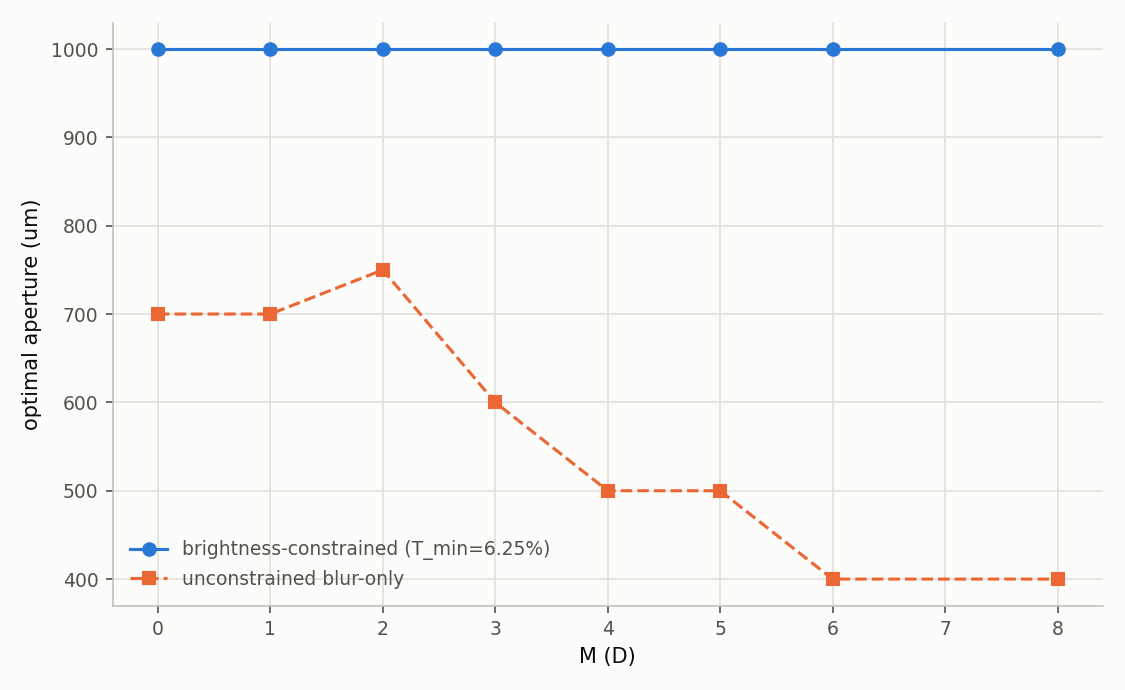
\includegraphics[width=0.85\textwidth]{figures/fig_stage3a_optimum_vs_M.png}
\caption{Brightness-constrained optimum aperture $a^\ast$ vs.\ myopia $M$, $T_{min}=6.25\%$, alongside the unconstrained (Chapter~\ref{ch:r1sweep}) optimum for comparison.}
\label{fig:stage3a-optimum}
\end{figure}

{\small
\begin{longtable}{rrrrr}
\caption{Brightness-constrained optimum, T\_min=6.25\%.}\label{tab:stage3a-full}\\
\toprule
M (D) & T\_min & a* (um) & r\_EE(50\%) at a* (um) & E\_rel at a* \\
\midrule
\endfirsthead
\multicolumn{5}{c}{\tablename\ \thetable\ -- continued}\\
\toprule
M (D) & T\_min & a* (um) & r\_EE(50\%) at a* (um) & E\_rel at a* \\
\midrule
\endhead
\bottomrule
\endfoot
0.0000 & 0.0625 & 1000.0000 & 7.3275 & 0.0625 \\
1.0000 & 0.0625 & 1000.0000 & 7.3275 & 0.0625 \\
2.0000 & 0.0625 & 1000.0000 & 10.1398 & 0.0625 \\
3.0000 & 0.0625 & 1000.0000 & 15.2893 & 0.0625 \\
4.0000 & 0.0625 & 1000.0000 & 21.7056 & 0.0625 \\
5.0000 & 0.0625 & 1000.0000 & 28.1338 & 0.0625 \\
6.0000 & 0.0625 & 1000.0000 & 34.9404 & 0.0625 \\
8.0000 & 0.0625 & 1000.0000 & 49.5132 & 0.0625 \\
\end{longtable}
}

\section{Result}

A single brightness floor of $6.25\%$ of full-pupil illuminance moves the optimum from
the unconstrained $400$--$750\um$ bracket ($r_{EE}(50\%)$, $M\le5\,$D) to $1000\um$ ---
much closer to the clinically observed bracket.

\textbf{An important caveat about the floor value itself, stated plainly.} The
$6.25$--$9\%$ figure was originally \emph{reverse-engineered} to reproduce the known
clinical range, not independently derived from a cited absolute-brightness threshold.
Chapter~\ref{ch:brightness_reconciliation} attempts exactly that independent
reconciliation, and reports it as still only partially resolved.

\section{All four blur percentiles under the same brightness constraint}
\label{sec:stage3a-all-percentiles}

Repeating this exact constrained optimization for $r_{EE}(70\%)$, $r_{EE}(80\%)$, and
$r_{EE}(90\%)$ --- at this same spot, using the identical $T_{min}=6.25\%$ floor and
the identical selection rule (smallest $r_{EE}(P)$ among apertures clearing the floor)
--- gives Figure~\ref{fig:stage3a-all-percentiles} and
Table~\ref{tab:stage3a-all-percentiles}.

\begin{figure}[htbp]
\centering
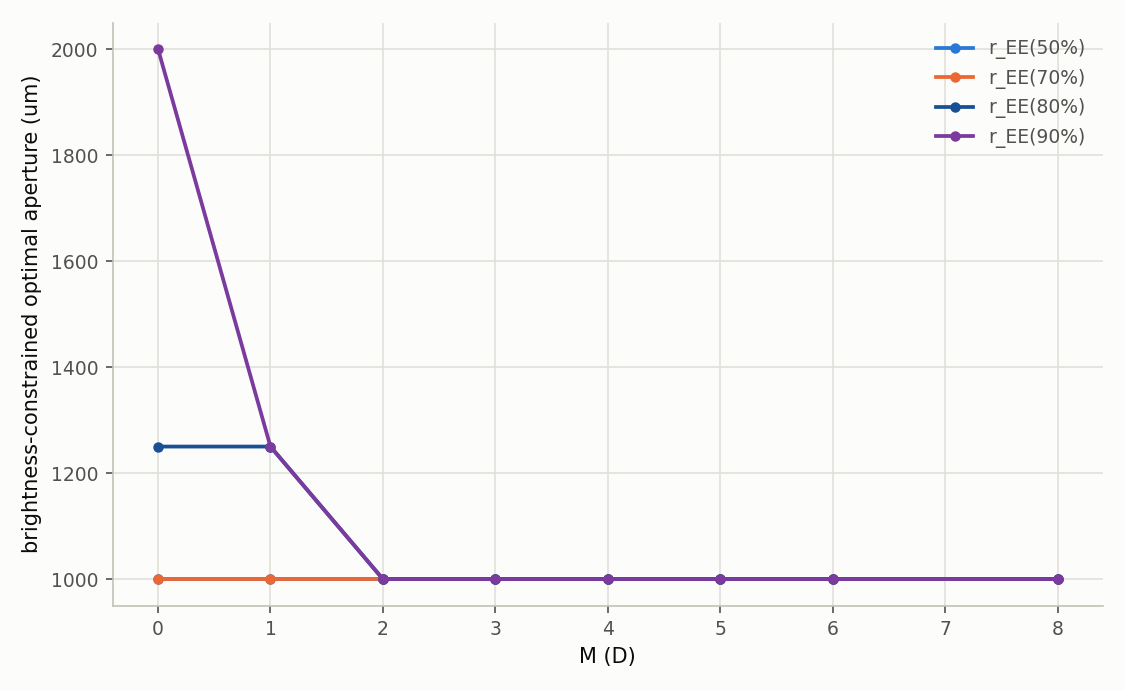
\includegraphics[width=0.85\textwidth]{figures/fig_stage3a_all_percentiles.png}
\caption{Brightness-constrained optimal aperture vs.\ myopia, all four blur percentiles, $T_{min}=6.25\%$.}
\label{fig:stage3a-all-percentiles}
\end{figure}

{\small
\begin{longtable}{rrrrr}
\caption{Brightness-constrained optimal aperture (um, T\_min=6.25\%), all four percentiles, per myopia level.}\label{tab:stage3a-all-percentiles}\\
\toprule
M (D) & r\_EE(50\%) & r\_EE(70\%) & r\_EE(80\%) & r\_EE(90\%) \\
\midrule
\endfirsthead
\multicolumn{5}{c}{\tablename\ \thetable\ -- continued}\\
\toprule
M (D) & r\_EE(50\%) & r\_EE(70\%) & r\_EE(80\%) & r\_EE(90\%) \\
\midrule
\endhead
\bottomrule
\endfoot
0 & 1000 & 1000 & 1250 & 2000 \\
1 & 1000 & 1000 & 1250 & 1250 \\
2 & 1000 & 1000 & 1000 & 1000 \\
3 & 1000 & 1000 & 1000 & 1000 \\
4 & 1000 & 1000 & 1000 & 1000 \\
5 & 1000 & 1000 & 1000 & 1000 \\
6 & 1000 & 1000 & 1000 & 1000 \\
8 & 1000 & 1000 & 1000 & 1000 \\
\end{longtable}
}

\textbf{A clean, generalizable finding, not visible from $r_{EE}(50\%)$ alone}: for
$M\ge2\,$D, \emph{all four percentiles converge to exactly the same optimal aperture}
($1000\um$) --- the brightness floor itself, not any property of the blur curve. This
is a direct, mechanical consequence of how the constrained search works: once the
\emph{unconstrained} optimum for a given percentile (Table~\ref{tab:r1-all-percentiles},
Section~\ref{sec:r1-all-percentiles}) already sits \emph{below} the floor aperture
($1000\um$ at $T_{min}=6.25\%$, $D_{pupil}=4000\um$), the constrained search is pushed
outward along the (still-decreasing, then floor-clipped) blur curve until it reaches
the floor itself and stops there --- so \emph{whenever the floor binds, which
percentile you optimize stops mattering entirely}. This only fails to hold at
$M=0$--$1\,$D, where $r_{EE}(80\%)$'s and $r_{EE}(90\%)$'s own \emph{unconstrained}
optima already sit at or above the floor (Table~\ref{tab:r1-all-percentiles}), so the
brightness constraint never binds for them and the constrained optimum simply equals
the unconstrained one.

\textbf{Practical reading}: at the myopia levels this project's own literature review
identifies as the clinically relevant range (moderate-to-high, $M\ge2\,$D), the choice
of blur-percentile metric --- one of this report's own recurring caveats
(Chapter~\ref{ch:percentile}) --- turns out not to matter for the brightness-constrained
design number at all, \emph{provided} the $6.25\%$ floor itself is trusted. The
remaining open question is therefore squarely the floor value, not the blur metric ---
exactly what Chapter~\ref{ch:brightness_reconciliation} investigates next.
